\chapter{Marco Teórico}

En este capítulo, se describen los fundamentos teóricos necesarios para el entendimiento y comprensión del proyecto. Se da una definición de los conceptos de robótica, robots, visión por computadora y la definición de las tareas realizadas por un robot autónomo para la navegación y ubicación de si mismo en un entorno. Se especifican las características técnicas del sistema Kinect y por último, se define la metodología Ágil para desarrollo de proyectos y los métodos PXP y Kanban para el desarrollo de aplicaciones, creando con esto una base teórica con la finalidad de tener una introducción del hardware y software utilizado, las herramientas de diseño y permitir al lector tener una idea de la naturaleza del contenido del resto del documento.

\section{Robótica}
La Robótica es aquella rama dentro de la Ingeniería que se ocupa de la aplicación de la informática al diseño y al uso de máquinas con el objetivo que de lo que de esto resulte pueda de alguna manera sustituir a las personas en la realización de determinadas funciones o tareas.
En palabras más simples, la robótica es la ciencia y la tecnología de los robots, porque básicamente se ocupa del diseño, manufactura y aplicaciones de los robots que crea. En la Robótica se combinan varias disciplinas al mismo tiempo, como la mecánica, la electrónica, la inteligencia artificial, la informática y la ingeniería de control, en tanto, también, por los quehaceres que desempeña, resulta fundamental el aporte que recibe y extrae de campos tales como el álgebra, los autómatas programables y las máquinas de estados.

\section{Robots}
El término robot alcanza su primera repercusión en la tercera década del siglo pasado, a instancias de R.U.R (robots Universal Rossum), una obra teatral de ciencia ficción escrita por el autor checo Karel Čapek, en la cual por primera vez se hace alusión al concepto de robot, extraído del término checo ``robota'', que significaba ``trabajos forzados''.

A su vez, el término ``robótica'' es acuñado por Isaac Asimov, definiendo a la ciencia que estudia a los robots. Asimov creó también las Tres Leyes de la Robótica, definidas de esta manera:

\begin{enumerate}
	\itemsep1pt \parskip1pt \parsep1pt
	\item Un robot no puede actuar contra un ser humano o, mediante la inacción, permitir que un ser humano sufra daños.
	\item Un robot debe obedecer las órdenes dadas por los seres humanos, salvo que estén en conflictos con la primera ley.
	\item Un robot debe proteger su propia existencia, a no ser que esté en conflicto con las dos primeras leyes.
\end{enumerate}

Desde sus comienzos como disciplina y como parte fundamental de la Ingeniería, la Robótica ha estado incansablemente buscando construir artefactos que materialicen el deseo humano de crear seres a su semejanza a quienes poder delegarles tareas, trabajos o actividades por demás pesadas y desagradables de llevar a cabo. Pero y aunque muchos ni se lo esperen, desde tiempos inmemoriales, muy, muy lejos de las computadoras, hubo unas cuantas expresiones de la robótica. Porque por ejemplo, los antiguos egipcios unieron brazos mecánicos a las estatuas de sus dioses y esgrimían que el movimiento de los miembros se llevaba a cabo por obra y gracias de estos, inclusive los griegos construyeron estatuas que operaban con sistemas hidráulicos, los cuales eran utilizados para fascinar a los adoradores de los templos.

Y también, aproximadamente entre los siglos XVII y XVIII, en Europa, se construyeron muñecos mecánicos muy ingeniosos que ostentaban algunas características como las que presentan los robots de la actualidad. En un constante e incansable ensayo a través de los siglos y cuando ya era un hecho la entrada en el nuevo milenio (2000), la empresa Honda Motor Co. Ltda. concretó a Asimo, el primer robot humanoide capaz de desplazarse de forma bípeda e interactuar con las personas.

La historia de la robótica va unida a la construcción de ``artefactos'', que trataban de materializar el deseo humano de crear seres a su semejanza y que lo descargasen del trabajo. El ingeniero español Leonardo Torres Quevedo (que construyó el primer mando a distancia para su automóvil mediante telegrafía sin hilo, el ajedrecista automático, el primer transbordador aéreo y otros muchos ingenios) acuñó el término ``automática'' en relación con la teoría de la automatización de tareas tradicionalmente asociadas.

\subsection{Clasificación de los robots}

En términos generales, un robot se clasifica por sus capacidades, así como también su área de operación, sus grados de autonomía o el fin con el que han sido construidos. Sin embargo, también pueden clasificarse en términos de la era en la que fue implementado, según su forma de construcción o la manera como son controlados. A continuación se exponen algunas formas comunes de clasificación:

\subsubsection{Según su cronología}
La que a continuación se presenta es la clasificación más común, respecto al área de robótica industrial:

\begin{description}
\item[1\textordfeminine\ Generación.]
Manipuladores. Son sistemas mecánicos multifuncionales con un sencillo sistema de control, bien manual, de secuencia fija o de secuencia variable.

\item[2\textordfeminine\ Generación.]
Robots de aprendizaje. Repiten una secuencia de movimientos que ha sido ejecutada previamente por un operador humano. El modo de hacerlo es a través de un dispositivo mecánico. El operador realiza los movimientos requeridos mientras el robot le sigue y los memoriza.

\item[3\textordfeminine\ Generación.]
Robots con control sensorizado. El controlador es una computadora que ejecuta las órdenes de un programa y las envía al manipulador para que realice los movimientos necesarios.

\item[4\textordfeminine\ Generación.]
Robots inteligentes. Son similares a los anteriores, pero además poseen sensores que envían información a la computadora de control sobre el estado del proceso. Esto permite una toma inteligente de decisiones y el control del proceso en tiempo real.
\end{description}

\subsubsection{Según su arquitectura}
La arquitectura, es definida por el tipo de configuración general del robot, puede ser metamórfica. El concepto de metamorfismo, de reciente aparición, se ha introducido para incrementar la flexibilidad funcional de un robot a través del cambio de su configuración por el propio robot.
El metamorfismo admite diversos niveles, desde los más elementales (cambio de herramienta o de efecto terminal), hasta los más complejos como el cambio o alteración de algunos de sus elementos o subsistemas estructurales.

Los dispositivos y mecanismos que pueden agruparse bajo la denominación genérica del robot, tal como se ha indicado, son muy diversos y es por tanto difícil establecer una clasificación coherente de los mismos que resista un análisis crítico y riguroso. La subdivisión de los robots, con base en su arquitectura, se hace en los siguientes grupos: poliarticulados, móviles, androides, zoomórficos e híbridos.

\begin{enumerate}
	\itemsep1pt \parskip1pt \parsep1pt
	\item Poliarticulados
	En este grupo se encuentran los robots de muy diversa forma y configuración, cuya característica común es la de ser básicamente sedentarios (aunque excepcionalmente pueden ser guiados para efectuar desplazamientos limitados) y estar estructurados para mover sus elementos terminales en un determinado espacio de trabajo según uno o más sistemas de coordenadas, y con un número limitado de grados de libertad. En este grupo, se encuentran los manipuladores, los robots industriales, los robots cartesianos y se emplean cuando es preciso abarcar una zona de trabajo relativamente amplia o alargada, actuar sobre objetos con un plano de simetría vertical o reducir el espacio ocupado en el suelo.

	\item Móviles
	Son robots basados en carros o plataformas, dotados de un sistema locomotor de tipo rodante y con gran capacidad de desplazamiento. Siguen su camino por telemando, guiándose por la información recibida de su entorno a través de sus sensores, a travès de rutas o movimientos previamente planificadas y un híbrido entre estas dos últimas.

	\item Androides
	Son robots que intentan reproducir total o parcialmente la forma y el comportamiento cinemático del ser humano. Actualmente, los androides son todavía dispositivos muy poco evolucionados y sin utilidad práctica, y destinados, fundamentalmente, al estudio y experimentación. Uno de los aspectos más complejos de estos robots, y sobre el que se centra la mayoría de los trabajos, es el de la locomoción bípeda. En este caso, el principal problema es controlar dinámica y coordinadamente en el tiempo real el proceso y mantener simultáneamente el equilibrio del robot.

	\item Zoomórficos
	Los robots zoomórficos, que considerados en sentido no restrictivo podrían incluir también a los androides, constituyen una clase caracterizada principalmente por sus sistemas de locomoción que imitan a los diversos seres vivos. A pesar de la disparidad morfológica de sus posibles sistemas de locomoción es conveniente agrupar a los robots zoomórficos en dos categorías principales: caminadores y no caminadores. El grupo de los robots zoomórficos no caminadores está muy poco evolucionado. Los experimentos efectuados en Japón basados en segmentos cilíndricos biselados acoplados axialmente entre sí y dotados de un movimiento relativo de rotación. Los robots zoomórficos caminadores multípedos son muy numerosos y están siendo objeto de experimentos en diversos laboratorios con vistas al desarrollo posterior de verdaderos vehículos terrenos, piloteados o autónomos, capaces de evolucionar en superficies muy accidentadas. Las aplicaciones de estos robots serán interesantes en el campo de la exploración espacial y en el estudio de los volcanes.

	\item Híbridos
	Corresponden a aquellos de difícil clasificación, cuya estructura se sitúa en combinación con alguna de las anteriores ya expuestas, bien sea por conjunción o por yuxtaposición. Por ejemplo, un dispositivo segmentado articulado y con ruedas, es al mismo tiempo, uno de los atributos de los robots móviles y de los robots zoomórficos.
\end{enumerate}

\subsubsection{Según su modalidad de control}
La modalidad de control se refiere a la dependencia –o no– de un operador humano que instruya órdenes al robot; por tanto, se subdivide en dos grandes grupos:

\begin{enumerate}
	\itemsep1pt \parskip1pt \parsep1pt
	\item Teledirigidos
	Se define como robots teledirigidos a aquellos que necesitan la intervención de un operador humano, ya sea en forma parcial o total, por ejemplo los utilizados en la desactivación de explosivos. Es necesario destacar que algunos investigadores sugieren que el término robot no es adecuado cuando estos dispositivos son teledirigidos.
	\item Autónomos
	Se les llama autónomos a aquellos robots que son capaces de tomar sus propias decisiones basados en la comprensión del entorno en que se encuentren. Existen numerosos tipos de robots de variadas configuraciones que se encuadran en esta categoría, como es el caso de un brazo robot con visión artificial sin asistencia humana realizando tareas de clasificación de objetos, o de los robots móviles del tipo vehículo.
\end{enumerate}

\subsection{Robots Autónomos}
Un robot autónomo es un robot que realiza comportamientos o tareas con un alto grado de autonomía, que es particularmente deseable en campos tales como la exploración del espacio, la limpieza de suelos, cortar el césped, y el tratamiento de aguas residuales.

Algunos robots de fábricas modernas son ``autónomos'' dentro de los límites estrictos de su entorno directo. Puede que no sea la existencia de todos los grados de libertad en su entorno, pero el lugar de trabajo del robot de la fábrica es un reto y, a menudo puede contener, variables caóticas e impredecibles. La orientación exacta y la posición del siguiente objeto de trabajo e incluso (en las fábricas más avanzadas) el tipo de objeto y la tarea requerida debe ser determinado. Esto puede variar de manera impredecible (por lo menos desde el punto de vista del robot).

Un área importante de la investigación robótica es permitir que el robot pueda hacer frente a su entorno ya sea en tierra, bajo el agua, en el aire, bajo tierra o en el espacio.

Un robot completamente autónomo puede:

\begin{itemize}
	\itemsep1pt \parskip1pt \parsep1pt
	\item Obtener información sobre el medio ambiente (Regla \#1)
	\item Trabajar por un período prolongado sin intervención humana (Regla \#2)
	\item Mover todo o parte de sí mismo a través de su entorno operativo sin ayuda humana (Regla \#3)
	\item Evitar situaciones que son perjudiciales para las personas, los bienes, o sí mismo, si esos son parte de sus especificaciones de diseño (Regla \#4)
\end{itemize}

Un robot autónomo también puede aprender o adquirir nuevos conocimientos como ajustarse a nuevos métodos para llevar a cabo sus tareas o adaptarse a un entorno cambiante.

Al igual que otras máquinas, los robots autónomos todavía requieren de un mantenimiento regular.

Ejemplos:

\subsubsection{Automantenimiento}
El primer requisito para la autonomía física completa es la capacidad de un robot para cuidar de sí mismo. Muchos de los robots que funcionan con baterías en el mercado hoy en día pueden encontrar y conectarse a una estación de carga, y algunos juguetes como Aibo de Sony son capaces de realizar auto-acoplamiento para cargar sus baterías.

El mantenimiento realizado se basa en la ``propiocepción'', o la capacidad de sentir el propio estado interno. En el ejemplo de carga de la batería, el robot puede decir propioceptivamente que sus baterías están bajas y en consecuencia, buscar el cargador. Otro sensor propioceptivo es común para la supervisión de calor. El aumento de la propiocepción se requerirá para los robots para trabajar de forma autónoma, cerca de la gente y en ambientes hostiles. Las propiocepciones comunes incluyen sensores de detección térmica, óptica y háptica, así como el efecto Hall (eléctrica).

\subsubsection{Sintiendo el medio ambiente}
La exterocepción es la detección de información del medio ambiente. Los robots autónomos deben tener una gama de sensores ambientales para llevar a cabo su tarea y no meterse en problemas.

Los sensores exteroceptivos comunes incluyen el espectro electromagnético, el sonido, el tacto, química (olor), la temperatura, la distancia hacia múltiples objetos, y la altitud.
Algunas cortadoras de césped robóticas adaptarán su programación mediante la detección de la velocidad en la que la hierba crece a medida que sea necesario para mantener un césped perfectamente cortado, y algunos robots de limpieza por aspiración toemem detectores de tierra que detectan la cantidad de suciedad que se está recogido y utilizan esta información para decirles que deben permanecer en un área durante más tiempo.

\subsubsection{Desempeño de tareas}
El siguiente paso en el comportamiento autónomo es para llevar a cabo realmente una tarea física. Una nueva área que muestra promesa comercial es la de los robots domésticos, con una avalancha de pequeños robots aspiradora que comienzan con iRobot y Electrolux en 2002 Mientras que el nivel de inteligencia no es muy alta en estos sistemas, que navegan en zonas extensas y conducen en situaciones estrechas alrededor de los hogares utilizando sensores de contacto y sin contacto. Ambos robots utilizan algoritmos propietarios para aumentar la cobertura por encima del simple rebote al azar.

El siguiente nivel de ejecución de la tarea autónoma requiere que un robot pueda realizar tareas condicionales. Por ejemplo, los robots de seguridad se pueden programar para detectar intrusos y responder de una manera particular, dependiendo de donde esté ubicado el intruso.

\subsubsection{Navegación interior}
Para que un robot pueda asociar comportamientos con un lugar (localización) requiere saber dónde está y ser capaz de navegar de punto a punto. Tal navegación comenzó mediante guía cableada en la década de 1970 y progresó en la década de 2000 a la triangulación mediante balizas. Los robots autónomos comerciales actuales navegan basándose en la detección de caraterísticas naturales.

Los primeros robots comerciales en lograrlo fueron el robot de hospital HelpMate de Pyxus y el robot guardia CyberMotion, ambos diseñados por pioneros en robótica en la década de 1980. Estos robots utilizaban originalmente planos de piso CAD creados manualmente, detección mediante sonar y variaciones de seguimiento de paredes para navegar a través de edificios. La próxima generación, tales como PatrolBot y la silla de ruadas autónoma de MobileRobots, ambos introducidos en 2004, tienen la capacidad de crear sus propios mapas basados en láser de un edificio y navegar por zonas abiertas, así como corredores. Su sistema de control cambia su ruta sobre la marcha si algo bloquea el camino.

Inicialmente, la navegación autónoma se basaba en sensores planares, como los telémetros láser, que sólo pueden realizar detecciones en un plano o nivel. Los sistemas más avanzados ahora fusionan la información de diversos sensores, tanto para la localización (posición) y la navegación. Los sistemas tales como Motivity pueden contar con diferentes sensores en diferentes áreas, dependiendo de lo que proporcione los datos más fiables en el momento, y pueden volver a generar mapas de entorno de forma autónoma.

En lugar de subir escaleras, lo que requiere hardware altamente especializado, la mayoría de los robots de interior navegan en áreas accesibles para minusválidos, controlando ascensores y puertas electrónicas. Con este tipo de interfaces de control de acceso, los robots ya pueden navegar libremente en el interior. Subir o bajar escaleras de forma autónoma y abrir puertas de forma manual, son temas actuales de investigación.

A medida que estas técnicas en interiores se siguen desarrollando, los robots aspiradora adquirirán la capacidad de limpiar una habitación específica designada por el usuario o una planta entera. Los robots de seguridad podrán rodear intrusos de forma cooperativa e incluso cortarles las salidas. Estos avances también traen protecciones asociadas: los mapas internos de los robots permiten típicamente la definición de ``zonas prohibidas'' para evitar que los mismos entren de forma autónoma en ciertas regiones.

\paragraph{Navegación en exteriores}
La autonomía al aire libre se logra más fácilmente en el aire, ya que los obstáculos son raros. Los misiles de crucero son robots altamente autónomas y bastante peligrosos. Los aviones no tripulados se utilizan cada vez más para el reconocimiento. Algunos de estos vehículos aéreos no tripulados (UAV) son capaces de volar toda su misión sin ninguna interacción humana en absoluto, excepto posiblemente para el aterrizaje cuando una persona interviene mediante control remoto por radio. Sin embargo, algunos aviones son capaces de realizar aterrizajes automáticos y seguros.

La autonomía al aire libre es más difícil para los vehículos de tierra, debido a:

\begin{itemize}
	\itemsep1pt \parskip1pt \parsep1pt
	\item La tridimensionalidad del terreno,
	\item Grandes disparidades en la densidad de superficie
	\item Exigencias climáticas
	\item Inestabilidad del medio ambiente detectado
\end{itemize}

En Estados Unidos, el proyecto MDARS (Mobile Detection Assessment and Response System), que definió y construyó un robot prototipo de vigilancia exterior en la década de 1990, se está llevando a producción y será implementado en 2006. El robot MDARS de General Dynamics puede navegar de forma semi-autónoma y detectar intrusos, utilizando la arquitectura de software MRHA (Multiple Robot Host Architecture) planeada para todos los vehículos militares no tripulados. El robot Seekur fue el primer robot comercial para demostrar las capacidades similares a MDARS para uso general por los aeropuertos, plantas de servicios públicos, instalaciones correccionales y Seguridad Nacional.

Los rovers MER-A y MER-B (conocidos actualmente como los rovers Spirit y Opportunity) pueden encontrar la posición del sol y navegar sus propias rutas a destinos sobre la marcha a través de:

\begin{itemize}
	\itemsep1pt \parskip1pt \parsep1pt
	\item Cartografía de la superficie mediante visión en 3D
	\item Cálculo de zonas seguras e inseguras en la superficie dentro de ese campo de visión
	\item Cálculo de rutas óptimas en toda la zona segura hacia el destino deseado
	\item Conducción a lo largo de la ruta calculada
	\item La repetición de este ciclo hasta que el destino se alcanza, o no haya ninguna ruta conocida hacia el destino
\end{itemize}

El Rover de ESA en planificación, ExoMars Rover, es capaz de localización relativa basada en visión y localización absoluta para navegar de forma autónoma a trayectorias seguras y eficaces a objetivos a través de:

\begin{itemize}
	\itemsep1pt \parskip1pt \parsep1pt
	\item La reconstrucción de modelos 3D del terreno que rodea al Rover con un par de cámaras estéreo
	\item La determinación de las zonas seguras e inseguras del terreno y la ``dificultad'' general para el Rover para navegar por el terreno
	\item Cálculo de caminos eficientes a través de la zona de seguridad hacia el destino deseado
	\item Conducir el Rover a lo largo del camino planeado
	\item La creación de un mapa de navegación de todos los datos de navegación anterior
\end{itemize}

El DARPA Grand Challenge y DARPA Urban Challenge han alentado el desarrollo de capacidades aún más autónomas para vehículos de tierra, mientras que este ha sido el objetivo demostrado por robots aéreos desde 1990 como parte de la AUVSI Internacional Aerial Robotics Competition.

\section{SLAM}
Para un robot autónomo, capaz de navegar por si mismo en un entorno, una de las tareas más desafiantes que puede realizar es la de estimar su posición y orientación en el ambiente en el cual navega, especialmente si no se cuenta con información previa sobre ese ambiente. De esto se trata SLAM, acrónimo en inglés para Simultaneous Localization And Mapping, o Localización y Mapeo Simultáneos.

\subsection{Introducción}
El problema de construcción de mapas y localización simultáneos pregunta si es posible que un vehículo autónomo comience en una ubicación desconocida dentro de un entorno desconocido y que construya de forma incremental un mapa de este entorno mientras que usa este mapa de forma simultánea para calcular de forma absoluta la localización o ubicación del vehículo.

La solución para este problema es, en múltiples aspectos, el ``Santo Grial'' de la comunidad de investigación de vehículos autónomos. Por ello, la principal ventaja de SLAM es que elimina la necesidad de infraestructuras artificiales o de poseer conocimiento topográfico a priori del entorno.

\subsection{Historia}
El problema general de SLAM ha sido objeto de considerable investigación desde el inicio de una comunidad de investigación de la robótica y de hecho antes de este en áreas como sistemas de navegación de vehículos tripulados y estudios geofísicos. Se han propuesto varios enfoques para abordar tanto el problema de SLAM y también problemas de navegación más simplificados donde se hacen disponible informaciones adicionales de mapa o de ubicación del vehículo.

En términos generales, estos enfoques adoptan una de tres filosofías principales. La más popular de ellas es la aproximación estimación-teoría o basada en el filtro de Kalman. La popularidad de este enfoque se debe a dos factores principales. En primer lugar, proporciona directamente tanto una solución recursiva para el problema de navegación y de una manera de computar estimaciones consistentes para la incertidumbre en ubicaciones de vehículos y referencias de mapas sobre la base de modelos estadísticos para el movimiento del vehículo y observaciones relativas de referencias. En segundo lugar, un corpus sustancial del método y la experiencia ha sido desarrollado en el sector aeroespacial, marítimo y otras aplicaciones de navegación, de las que la comunidad autónoma de vehículos puede extraer.

Una segunda filosofía es la de evitar la necesidad de estimaciones de posición absoluta y de medidas precisas de la incertidumbre y en lugar de ello, emplear conocimiento más cualitativo de la ubicación relativa de las referencias y el vehículo para construir mapas y guiar el movimiento. El enfoque cualitativo para la navegación y el problema general de SLAM tiene muchas ventajas potenciales sobre la metodología de estimación-teoría en términos de limitar la necesidad de modelos precisos y los requisitos computacionales resultantes, y en su significativo ``atractivo antropomórfico''.

La tercera y muy amplia filosofía, elimina el filtro de Kalman o el riguroso formalismo estadístico al tiempo que conserva un enfoque esencialmente numérico o computacional para el problema de navegación y SLAM. Tales enfoques incluyen el uso de pareos de lugares de interés icónicos, el registro de un mapa global, regiones delimitadas y otras medidas para describir la incertidumbre. Un trabajo notable en esta filosofía se ha realizado mediante el uso de un enfoque bayesiano para mapeo de edificios que no asume las distribuciones de probabilidad de Gauss como es requerido por el filtro de Kalman. Esta técnica, aunque muy eficaz para la localización con respecto a los mapas, no se presta para proporcionar una solución gradual a SLAM, donde un mapa se construye gradualmente a medida que se recibe información de los sensores.
\cite{dissanayake01solution}

\section{Visión por Computadora}
Es el campo de la Inteligencia Artificial enfocado a que las computadoras puedan extraer información a partir de imágenes, ofreciendo soluciones a problemas del mundo real. La visión para los humanos no es ningún problema, pero para las máquinas es un campo muy complicado. Influyen texturas, luminosidad, sombras, objetos complejos, etc.

El propósito de la visión artificial o por computadora, es programar un computador para que ``entienda'' una escena o las características de una imagen.

Los objetivos típicos de la visión artificial incluyen:

\begin{itemize}
	\itemsep1pt \parskip1pt \parsep1pt
	\item La detección, segmentación, localización y reconocimiento de ciertos objetos en imágenes (por ejemplo, caras humanas).
	\item La evaluación de los resultados (por ejemplo, segmentación, registro).
	\item Registro de diferentes imágenes de una misma escena u objeto, es decir, hacer concordar un mismo objeto en diversas imágenes.
	\item Seguimiento de un objeto en una secuencia de imágenes.
	\item Mapeo de una escena para generar un modelo tridimensional de la escena; este modelo podría ser usado por un robot para navegar por la escena.
	\item Estimación de las posturas tridimensionales de humanos.
	\item Búsqueda de imágenes digitales por su contenido.
\end{itemize}

Estos objetivos se consiguen por medio de reconocimiento de patrones, aprendizaje estadístico, geometría de proyección, procesamiento de imágenes, teoría de grafos y otros campos. La visión artificial cognitiva está muy relacionada con la psicología cognitiva y la computación biológica.

\section{Microsoft Kinect}
Kinect para Xbox 360, o simplemente Kinect (originalmente conocido por el nombre en clave ``Project Natal''), es un controlador de juego libre y entretenimiento creado por Alex Kipman, desarrollado por Microsoft para las videoconsolas Xbox 360 y Xbox One, y desde junio del 2011 para PC a través de Windows 7 y Windows 8.

Kinect permite a los usuarios controlar e interactuar con la consola sin necesidad de tener contacto físico con un controlador de videojuegos tradicional, mediante una interfaz natural de usuario que reconoce gestos, comandos de voz, y objetos e imágenes. El dispositivo tiene como objetivo primordial aumentar el uso de la Xbox 360, más allá de la base de jugadores que posee en la actualidad.

En sí, Kinect compite con los sistemas Wiimote con Wii MotionPlus y PlayStation Move, que también controlan el movimiento para las consolas Wii y PlayStation 3, respectivamente.

El nombre en clave ``Proyecto Natal'' responde a la tradición de Microsoft de utilizar ciudades como nombres en clave. Alex Kipman, director de Microsoft, quien incubó el proyecto, decidió ponerle el nombre de la ciudad brasileña Natal como un homenaje a su país de origen y porque la palabra natal significa ``de o en relación al nacimiento'', lo que refleja la opinión de Microsoft en el proyecto como ``el nacimiento de la próxima generación de entretenimiento en el hogar''. Poco antes de la E3 2010 varios weblogs tropezaron con un anuncio que supuestamente se filtró en el sitio italiano de Microsoft de que sugirió el título ``Kinect'', que confirmó más tarde.

\begin{figure}[h]
\centering
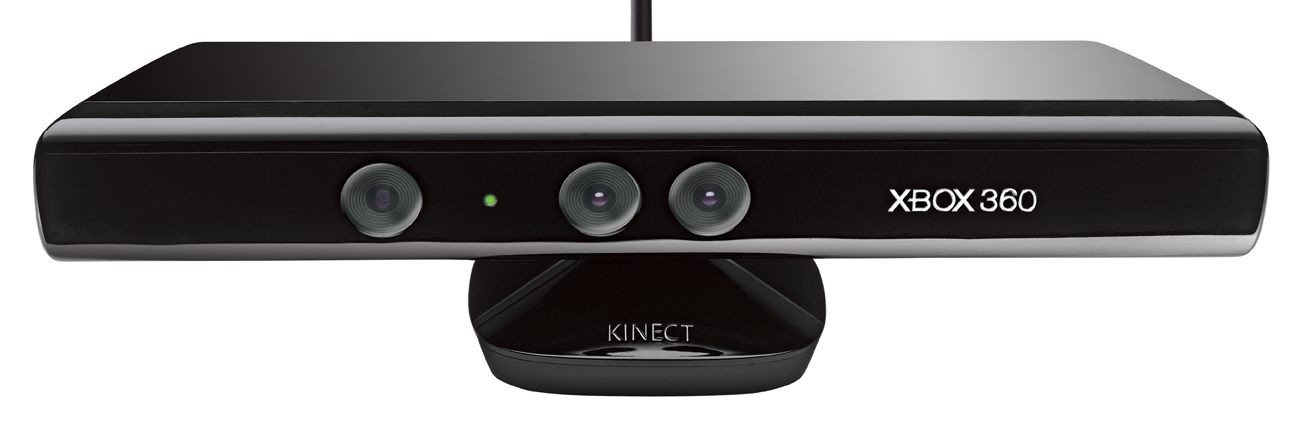
\includegraphics[width=0.75\textwidth]{kinectxbox360}
\caption{Microsoft XBOX 360 Kinect}
\end{figure}

\subsection{Características}
El sensor de Kinect es una barra horizontal de aproximadamente 23 cm (9 pulgadas) conectada a una pequeña base circular con un eje de articulación de rótula, y está diseñado para ser colocado longitudinalmente por encima o por debajo de la pantalla de vídeo.

El dispositivo cuenta con una cámara RGB, un sensor de profundidad, un micrófono de múltiples matrices y un procesador personalizado que ejecuta el software patentado, que proporciona captura de movimiento de todo el cuerpo en 3D, reconocimiento facial y capacidades de reconocimiento de voz.

\begin{figure}[h]
\centering
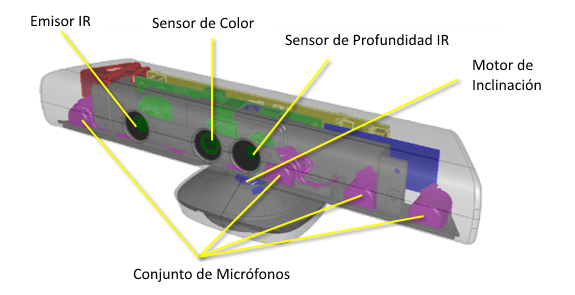
\includegraphics[width=0.75\textwidth]{kinectcomponents}
\caption{Componentes del Kinect}
\end{figure}

El sensor contiene un mecanismo de inclinación motorizado y en caso de usar una PC o un modelo original de Xbox 360, tiene que ser conectado a una toma de corriente a través de un adaptador, ya que la corriente que puede proveerle el cable USB es insuficiente; para el caso del modelo de Xbox 360 S esto no es necesario ya que esta consola cuenta con una toma especialmente diseñada para conectar el Kinect y esto permite proporcionar la corriente necesaria que requiere el dispositivo para funcionar correctamente.

El sensor de profundidad es un proyector de infrarrojos combinado con un sensor CMOS monocromo que permite a Kinect ver la habitación en 3D en cualquier condición de luz ambiental. El rango de detección de la profundidad del sensor es ajustable gracias al software de Kinect capaz de calibrar automáticamente el sensor.

\subsection{Especificaciones Técnicas}
Sus especificaciones \cite{openkinecthardware} \cite{ifixitkinect} más relevantes son:

\begin{itemize}
	\itemsep1pt \parskip1pt \parsep1pt
	\item Cámara / sensor infrarrojo: Microsoft / X853750001 / VCA379C7130 / MT9M001
	\item Rango efectivo (aproximado): 1,2m – 3,5m (puede ser menor o mayor, dependiendo de las condiciones ambientales)
	\item Resolución: 640x480 píxeles @ 30 Hz (profundidad de 11 bits: 2048 niveles de sensibilidad)
	\item Cámara RGB: VNA38209015 / MT9M112 / MT9v112
	\item Resolución: 640x480 píxeles @ 30 Hz (VGA de 8 bits)
	\item Emisor / proyector infrarrojo: OG12 / 0956 / D306 / JG05A
	\item Proyector láser de 830 nm.
	\item Potencia de salida: 60\~ mW
\end{itemize}

\subsection{Requerimientos para uso en Robótica}

El Kinect requiere 12 voltios \cite{openkinecthardware} para su funcionamiento (8 V como mínimo); es por ello que, tal como se mencionó anteriormente, la versión para PC cuenta con un adaptador de voltaje adicional, ya que el voltaje proporcionado por la conexión USB es por especificación de 5 voltios.

Es posible encontrar diversos tutoriales en línea \cite{batterypoweredkinect} sobre cómo alimentar al Kinect con la energía necesaria para manejarlo desde un robot autónomo y eliminar la necesidad de utilizar una extensión, asistiendo en su transportabilidad.

\section{Desarrollo Ágil de Proyectos}

En todo proyecto, el objetivo deseado es (o debería ser) el de maximizar la eficiencia y disminuir el costo, ya sea monetario o de tiempo. Para lograr este objetivo se han propuesto diferentes formas de administrar o gerenciar los proyectos, con infinidad de niveles de control, desde prácticamente ningún control en lo absoluto, hasta la microgerencia de las tareas más mínimas posibles.

El desarrollo de un trabajo especial de grado, tesis, o proyecto de grado puede verse, tal como se denominó por último, como un proyecto en si mismo, donde el objetivo es cumplir con los objetivos generales y específicos dentro de un marco de tiempo determinado, por lo que puede aplicarse lo mencionado al inicio para cumplir con los objetivos de la mejor manera posible.

Así pues, en el área de la ingeniería de sistemas y el desarrollo de software, se han empleado igualmente innumerables métodos para llevar a cabo la gerencia de un proyecto; sin que esto pretenda convertirse en un estudio a profundidad de dichos métodos, se nombra a continuación uno de los más populares en la actualidad, junto algunos métodos que emplean su filosofía y cuyo fin no es otro que el de organizar el desarrollo del proyecto y así poder rendir cuentas del mismo.

Las metodologías Ágiles de desarrollo, fueron propuestas en el año 2001 por diversos representantes de múltiples metodologías de desarrollo, tales como SCRUM, Programación Extrema, DSOM, Desarrollo de Software Adaptativo, Crystal y otros, con el fin de encontrar un terreno común que involucrara una alternativa al desarrollo de software pesado y orientado a la documentación.

Su idea consistió en enfocar el proceso de desarrollo en las personas en vez de al proceso en sí, reduciendo la burocracia y los procesos de planificación, documentación y modelado al mínimo posible, a través de principios documentados en un ``manifiesto''.

\subsection{Principios del Desarrollo Ágil}

El manifiesto para el Desarrollo Ágil de Software, indica el enfoque a seguir por esta metodología. Sus valores principales son los siguientes:

\begin{itemize}
	\itemsep1pt \parskip1pt \parsep1pt
	\item Individuos e interacciones sobre procesos y herramientas
	\item Software funcionando sobre documentación extensiva
	\item Colaboración con el cliente sobre negociación contractual
	\item Respuesta ante el cambio sobre seguir un plan
\end{itemize}

En las propias palabras del manifiesto: ``Esto es, aunque valoramos los elementos de la derecha, valoramos más los de la izquierda''.\cite{beck2001manifiesto}

Los principios producto de estos valores son:\cite{beck2001principios}

\begin{itemize}
	\itemsep1pt \parskip1pt \parsep1pt
	\item Nuestra mayor prioridad es satisfacer al cliente mediante la entrega temprana y continua de software con valor.
	\item Aceptamos que los requisitos cambien, incluso en etapas tardías del desarrollo. Los procesos Ágiles aprovechan el cambio para proporcionar ventaja competitiva al	cliente.
	\item Entregamos software funcional frecuentemente, entre dos semanas y dos meses, con preferencia al periodo de tiempo más corto posible.
	\item Los responsables de negocio y los desarrolladores	trabajamos juntos de forma cotidiana durante todo el proyecto.
	\item Los proyectos se desarrollan en torno a individuos motivados. Hay que darles el entorno y el apoyo que necesitan, y confiarles la ejecución del trabajo.
	\item El método más eficiente y efectivo de comunicar información al equipo de desarrollo y entre sus miembros es la conversación cara a cara.
	\item El software funcionando es la medida principal de	progreso.
	\item Los procesos Ágiles promueven el desarrollo sostenible. Los promotores, desarrolladores y usuarios
	debemos ser capaces de mantener un ritmo constante de forma indefinida.
	\item La atención continua a la excelencia técnica y al	buen diseño mejora la Agilidad.
	\item La simplicidad, o el arte de maximizar la cantidad de	trabajo no realizado, es esencial.
	\item Las mejores arquitecturas, requisitos y diseños emergen de equipos auto-organizados.
	\item A intervalos regulares el equipo reflexiona sobre	cómo ser más efectivo para a continuación ajustar y perfeccionar su comportamiento en consecuencia.
\end{itemize}

\section{Personal Extreme Programming}
La programación extrema o \textit{eXtreme Programming} (XP) es una metodología de desarrollo de la ingeniería de software formulada por Kent Beck, autor del primer libro sobre la materia, \textit{Extreme Programming Explained: Embrace Change} (1999). Es el más destacado de los procesos ágiles de desarrollo de software. Al igual que éstos, la programación extrema se diferencia de las metodologías tradicionales principalmente en que pone más énfasis en la adaptabilidad que en la previsibilidad.

Los defensores de XP consideran que los cambios de requisitos sobre la marcha son un aspecto natural, inevitable e incluso deseable del desarrollo de proyectos. Creen que ser capaz de adaptarse a los cambios de requisitos en cualquier punto de la vida del proyecto es una aproximación mejor y más realista que intentar definir todos los requisitos al comienzo del proyecto e invertir esfuerzos después en controlar los cambios en los requisitos.

Se puede considerar la programación extrema como la adopción de las mejores metodologías de desarrollo de acuerdo a lo que se pretende llevar a cabo con el proyecto, y aplicarlo de manera dinámica durante el ciclo de vida del software.

\subsection{Características}
Las características fundamentales del método son:

\begin{itemize}
	\itemsep1pt \parskip1pt \parsep1pt
	\item Desarrollo iterativo e incremental: pequeñas mejoras, unas tras otras.
	\item Pruebas unitarias continuas, frecuentemente repetidas y automatizadas, incluyendo pruebas de regresión. Se aconseja escribir el código de la prueba antes de la codificación. Véase, por ejemplo, las herramientas de prueba JUnit orientada a Java, DUnit orientada a Delphi, NUnit para la plataforma.NET o PHPUnit para PHP. Estas tres últimas inspiradas en JUnit, la cual, a su vez, se inspiró en SUnit, el primer framework orientado a realizar tests, realizado para el lenguaje de programación Smalltalk.
	\item Programación en parejas: se recomienda que las tareas de desarrollo se lleven a cabo por dos personas en un mismo puesto. La mayor calidad del código escrito de esta manera -el código es revisado y discutido mientras se escribe- es más importante que la posible pérdida de productividad inmediata. En este sentido, la modalidad personal difiere por razones obvias; sin embargo, las demás características son perfectamente aplicables.
	\item Frecuente integración del equipo de programación con el cliente o usuario. Se recomienda que un representante del cliente trabaje junto al equipo de desarrollo.
	\item Corrección de todos los errores antes de añadir nueva funcionalidad. Hacer entregas frecuentes.
	\item Refactorización del código, es decir, reescribir ciertas partes del código para aumentar su legibilidad y mantenibilidad pero sin modificar su comportamiento. Las pruebas han de garantizar que en la refactorización no se ha introducido ningún fallo.
	\item Propiedad del código compartida: en vez de dividir la responsabilidad en el desarrollo de cada módulo en grupos de trabajo distintos, este método promueve el que todo el personal pueda corregir y extender cualquier parte del proyecto. Las frecuentes pruebas de regresión garantizan que los posibles errores serán detectados.
	\item Simplicidad en el código: es la mejor manera de que las cosas funcionen. Cuando todo funcione se podrá añadir funcionalidad si es necesario. La programación extrema apuesta que es más sencillo hacer algo simple y tener un poco de trabajo extra para cambiarlo si se requiere, que realizar algo complicado y quizás nunca utilizarlo.
\end{itemize}

La simplicidad y la comunicación son extraordinariamente complementarias. Con más comunicación resulta más fácil identificar qué se debe y qué no se debe hacer. Cuanto más simple es el sistema, menos tendrá que comunicar sobre éste, lo que lleva a una comunicación más completa, especialmente si se puede reducir el equipo de programadores.

\section{Kanban}

Kanban, del japonés \begin{CJK*}{UTF8}{gbsn}かんばん\end{CJK*}(\begin{CJK*}{UTF8}{gbsn}看板\end{CJK*}), que es literalmente ``letrero'' o ``cartelera'', es un sistema de programación para la producción \textit{Lean} y justo-a-tiempo.

Kanban se basa en una idea muy simple: el trabajo en curso (Work In Progress, WIP) debería limitarse, y sólo deberíamos empezar con algo nuevo cuando un bloque de trabajo anterior haya sido entregado o ha pasado a otra función posterior de la cadena. El Kanban (o tarjeta señalizadora) implica que se genera una señal visual para indicar que hay nuevos bloques de trabajo que pueden ser comenzados porque el trabajo en curso actual no alcanza el máximo acordado.

Kanban usa un mecanismo de control visual para hacer seguimiento del trabajo conforme este viaja a través del flujo de valor. Típicamente, se usa un panel o pizarra con notas adhesivas o un panel electrónico de tarjetas. Las mejores prácticas apuntan probablemente al uso de ambos.

Las metodologías Ágiles han obtenido buenos resultados proporcionando transparencia respecto al trabajo en curso y completado, así como en el reporte de métricas como la velocidad (cantidad de trabajo realizada en una iteración). Kanban sin embargo va un paso más allá y proporciona transparencia al proceso y su flujo. Kanban expone los cuellos de botella, colas, variabilidad y desperdicios. Todas las cosas que impactan al rendimiento de la organización en términos de la cantidad de trabajo entregado y el ciclo de tiempo requerido para entregarlo. Kanban proporciona a los miembros del equipo y a las partes interesadas visibilidad sobre los efectos de sus acciones (o falta de acción). De esta forma, los casos de estudios preliminares están demostrando que Kanban cambia el comportamiento y motiva a una mayor colaboración en el trabajo. La visibilidad de los cuellos de botella, desperdicios y variabilidades y su impacto también promueve la discusión sobre la posibles mejoras, y los equipos comienzan rápidamente a implementar mejoras en su proceso.\cite{Skarin201003}

\subsection{Trello}

Trello es una plataforma de software que utiliza el paradigma Kanban para el manejo de proyectos. Iniciado en el año 2011 por la compañía Fog Creek Software y caracterizado como software de productividad, este utiliza un sistema de tableros, listas y tarjetas para llevar el control de múltiples tipos de proyecto, sin estar limitado a proyectos de desarrollo de software, por lo cual es altamente versatil. Las tarjetas aceptan comentarios, archivos adjuntos, votos, fechas de entrega y listas de verificación.

Para este proyecto, se abrió un tablero en Trello accesible desde la dirección \url{https://trello.com/b/yIMdcTCR/tesis-ros-kinect}, cuyas listas representan un híbrido entre las disponibles en PXP y Kanban, de la siguiente manera:

\begin{itemize}
	\itemsep1pt \parskip1pt \parsep1pt
	\item Pendientes: Tareas que están por ser ejecutadas.
	\item Actuales: Tareas que están siendo ejecutadas actualmente.
	\item Entregadas: Tareas que están marcadas como realizadas, pero que no han sido verificadas aún.
	\item Rechazadas: Tareas que, habiendo sido entregadas, presentan alguna falla o requieren algún cambio, por lo cual se colocan en esta lista para ser revisadas.
	\item Listas: Tareas que han sido verificadas y aceptadas.
	\item Ideas: Tarjetas que representan ideas aplicar, o tareas que no pueden pasar a la lista ``Pendientes'' por no haber recursos disponibles para ellas.
\end{itemize}

\begin{figure}[ht]
\centering
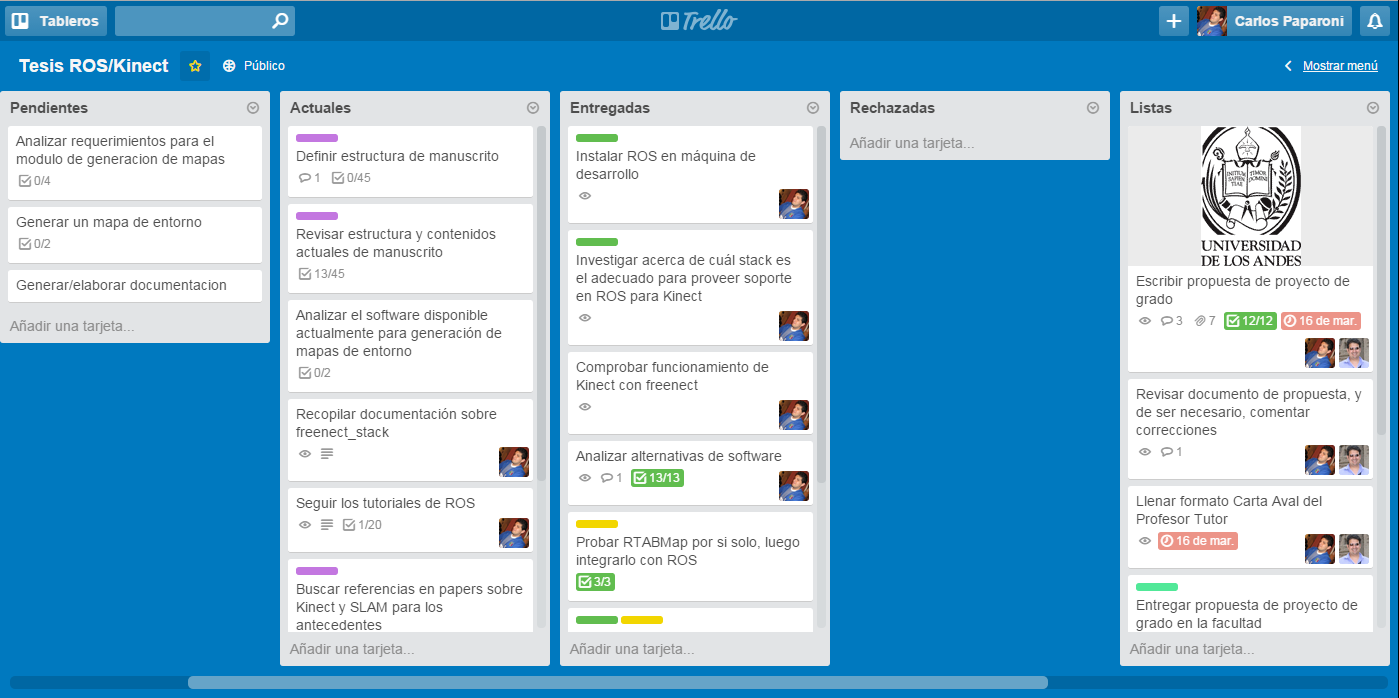
\includegraphics[width=1.00\textwidth]{trelloprojectwindow}
\caption{Tablero en Trello para el proyecto de grado}
\end{figure}

\subsubsection{Uso}

Cada tarea a realizar se coloca como una tarjeta en la lista correspondiente a ``Pendientes'' o ``Ideas'' según sea el caso, y una vez estén disponibles los recursos para tomarla (siendo estos recursos tiempo, o disponibilidad de la o las personas involucradas) se pasa dicha tarjeta, mediante arrastrar y colocar, a la lista de ``Actuales''. Esto permite ver el flujo de trabajo, tal como se mencionaba anteriormente, y permite saber el estado actual del proyecto si la tabla se mantiene actualizada.

Una vez terminada la tarea, se coloca en la lista ``Entregadas'', para su revisión (en el caso de este proyecto, el cliente del mismo viene a ser el profesor tutor, quien es la persona que puede verificar que se haya llevado a cabo satisfactoriamente o no). En caso que la tarea esté correcta, se puede pasar a la lista ``Listas'', lo cual marca la completación de la tarea, y la liberación de los recursos empleados para tomar nuevas tareas disponibles. En caso de observar algún error, la tarea pasa a la lista ``Rechazadas'', para su revisión y corrección.
